\documentclass[landscape,final,a0paper,fontscale=0.285]{baposter}

\usepackage{calc}
\usepackage{graphicx}
\usepackage{amsmath}
\usepackage{amssymb}
\usepackage{relsize}
\usepackage{multirow}
\usepackage{rotating}
\usepackage{bm}
\usepackage{url}

\usepackage{graphicx}
\usepackage{multicol}

\usepackage{palatino}

\newcommand{\captionfont}{\footnotesize}

\graphicspath{{images/}{../images/}}
\usetikzlibrary{calc}

\newcommand{\SET}[1]  {\ensuremath{\mathcal{#1}}}
\newcommand{\MAT}[1]  {\ensuremath{\boldsymbol{#1}}}
\newcommand{\VEC}[1]  {\ensuremath{\boldsymbol{#1}}}
\newcommand{\Video}{\SET{V}}
\newcommand{\video}{\VEC{f}}
\newcommand{\track}{x}
\newcommand{\Track}{\SET T}
\newcommand{\LMs}{\SET L}
\newcommand{\lm}{l}
\newcommand{\PosE}{\SET P}
\newcommand{\posE}{\VEC p}
\newcommand{\negE}{\VEC n}
\newcommand{\NegE}{\SET N}
\newcommand{\Occluded}{\SET O}
\newcommand{\occluded}{o}



%%%%%%%%%%%%%%%%%%%%%%%%%%%%%%%%%%%%%%%%%%%%%%%%%%%%%%%%%%%%%%%%%%%%%%%%%%%%%%%%
%%%% Some math symbols used in the text
%%%%%%%%%%%%%%%%%%%%%%%%%%%%%%%%%%%%%%%%%%%%%%%%%%%%%%%%%%%%%%%%%%%%%%%%%%%%%%%%

%%%%%%%%%%%%%%%%%%%%%%%%%%%%%%%%%%%%%%%%%%%%%%%%%%%%%%%%%%%%%%%%%%%%%%%%%%%%%%%%
% Multicol Settings
%%%%%%%%%%%%%%%%%%%%%%%%%%%%%%%%%%%%%%%%%%%%%%%%%%%%%%%%%%%%%%%%%%%%%%%%%%%%%%%%
\setlength{\columnsep}{1.5em}
\setlength{\columnseprule}{0mm}

%%%%%%%%%%%%%%%%%%%%%%%%%%%%%%%%%%%%%%%%%%%%%%%%%%%%%%%%%%%%%%%%%%%%%%%%%%%%%%%%
% Save space in lists. Use this after the opening of the list
%%%%%%%%%%%%%%%%%%%%%%%%%%%%%%%%%%%%%%%%%%%%%%%%%%%%%%%%%%%%%%%%%%%%%%%%%%%%%%%%
\newcommand{\compresslist}{%
\setlength{\itemsep}{1pt}%
\setlength{\parskip}{0pt}%
\setlength{\parsep}{0pt}%
}

%%%%%%%%%%%%%%%%%%%%%%%%%%%%%%%%%%%%%%%%%%%%%%%%%%%%%%%%%%%%%%%%%%%%%%%%%%%%%%
%%% Begin of Document
%%%%%%%%%%%%%%%%%%%%%%%%%%%%%%%%%%%%%%%%%%%%%%%%%%%%%%%%%%%%%%%%%%%%%%%%%%%%%%

\begin{document}

%%%%%%%%%%%%%%%%%%%%%%%%%%%%%%%%%%%%%%%%%%%%%%%%%%%%%%%%%%%%%%%%%%%%%%%%%%%%%%
%%% Here starts the poster
%%%---------------------------------------------------------------------------
%%% Format it to your taste with the options
%%%%%%%%%%%%%%%%%%%%%%%%%%%%%%%%%%%%%%%%%%%%%%%%%%%%%%%%%%%%%%%%%%%%%%%%%%%%%%
% Define some colors

% \definecolor{lightblue}{cmyk}{0.83,0.24,0,0.12}
\definecolor{lightblue}{rgb}{0.145,0.6666,1}

\definecolor{bgc_1}{RGB}{93, 194,232}
\definecolor{bgc_2}{RGB}{144, 190, 242}
\definecolor{hc_1}{RGB}{29,105,218}
\definecolor{hc_2}{RGB}{240,141,96}


\hyphenation{resolution occlusions}

\begin{poster}%
  % Poster Options
  {
  % Show grid to help with alignment
  grid=false,
  % Column spacing
  colspacing=1em,
  % Color style
  bgColorOne=bgc_2,
  bgColorTwo=white,
  borderColor=hc_1,
  headerColorOne=white,
  headerColorTwo=hc_1,
  headerFontColor=black,
  boxColorOne=hc_1,
  boxColorTwo=hc_2,
  % Format of textbox
  textborder=faded,
  % Format of text header
  eyecatcher=true,
  headerborder=open,
  headerheight=0.1\textheight,
%  textfont=\sc, An example of changing the text font
  headershape=roundedright,
  headershade=shadelr,
  headerfont=\Large\textsc, %Sans Serif
  textfont={\setlength{\parindent}{1.5em}},
  boxshade=shadelr,
%   background=shadetb, 
  background=shadelr, 
%   background=plain, 
  linewidth=0pt
  }
  % Eye Catcher
  {
  \vspace{0.8em}}
  % Title
  {
\includegraphics[height=1.8em]{images/title_v2.png}
  \textsc{
  }\vspace{-0.1em}}
  % Authors
  {{ Miguel Perez.Xochicale@gmail.com}\\
  } 
  % University logo
  {% The makebox allows the title to flow into the logo, this is a hack because of the L shaped logo.
  }

%%%%%%%%%%%%%%%%%%%%%%%%%%%%%%%%%%%%%%%%%%%%%%%%%%%%%%%%%%%%%%%%%%%%%%%%%%%%%%
%%% Now define the boxes that make up the poster
%%%---------------------------------------------------------------------------
%%% Each box has a name and can be placed absolutely or relatively.
%%% The only inconvenience is that you can only specify a relative position 
%%% towards an already declared box. So if you have a box attached to the 
%%% bottom, one to the top and a third one which should be in between, you 
%%% have to specify the top and bottom boxes before you specify the middle 
%%% box.
%%%%%%%%%%%%%%%%%%%%%%%%%%%%%%%%%%%%%%%%%%%%%%%%%%%%%%%%%%%%%%%%%%%%%%%%%%%%%%
    %
    % A coloured circle useful as a bullet with an adjustably strong filling
    \newcommand{\colouredcircle}{%
      \tikz{\useasboundingbox (-0.2em,-0.32em) rectangle(0.2em,0.32em); 
      \draw[draw=black,fill=lightblue,line width=0.03em] (0,0) circle(0.18em);}}

%%%%%%%%%%%%%%%%%%%%%%%%%%%%%%%%%%%%%%%%%%%%%%%%%%%%%%%%%%%%%%%%%%%%%%%%%%%%%%
  \headerbox{Introduction}{name=introduction,column=0,row=0}{
%%%%%%%%%%%%%%%%%%%%%%%%%%%%%%%%%%%%%%%%%%%%%%%%%%%%%%%%%%%%%%%%%%%%%%%%%%%%%%
The use of data from wearable sensors to analyse Human-Activity Recognition 
(e.g. walking, running, cycling, rowing, etc.) has incresed during the 
last 20 years. Nonetheless, when it comes to studying dextrous performance, 
recognition of event activities might not be sufficient. 

Dexterity in human activity is seldom an exclusive matter of performing events faster
or sequencing the events in a more consistent and defined manner, but could involve 
performing the actions in a very different way when compared to novices. 
Theferefore, identifying how \textit{well} an action is performed 
is more challenging than simply identifying action type \cite{nhammerla11}.

This research will extend the field of HAR by applying concepts from Chaos Theory \cite{asama13}  
to create novel analysis and interpretation of the data which allows us to recognise dexterity.
      \vspace{0.0em}
 }

 
%%%%%%%%%%%%%%%%%%%%%%%%%%%%%%%%%%%%%%%%%%%%%%%%%%%%%%%%%%%%%%%%%%%%%%%%%%%%%%
\headerbox{Research Questions}{name=questions,column=0,above=bottom}{
%%%%%%%%%%%%%%%%%%%%%%%%%%%%%%%%%%%%%%%%%%%%%%%%%%%%%%%%%%%%%%%%%%%%%%%%%%%%%%
\begin{itemize}\compresslist
   \item How can phase space representation quantify dexterity in human activities?
   \item How can we apply Takens's Theorem and Principal Components Analysis 
         to characterize Human Activities?
   \item How do concepts from nonlinear dynamics 
         help us to characterize dexterity in human activities?
   \end{itemize}
  }
  
%%%%%%%%%%%%%%%%%%%%%%%%%%%%%%%%%%%%%%%%%%%%%%%%%%%%%%%%%%%%%%%%%%%%%%%%%%%%%%
\headerbox{Phase Space Representation}{name=psr,column=0,below=introduction}{
%%%%%%%%%%%%%%%%%%%%%%%%%%%%%%%%%%%%%%%%%%%%%%%%%%%%%%%%%%%%%%%%%%%%%%%%%%%%%%
\vspace{0.5em}

\noindent{\centering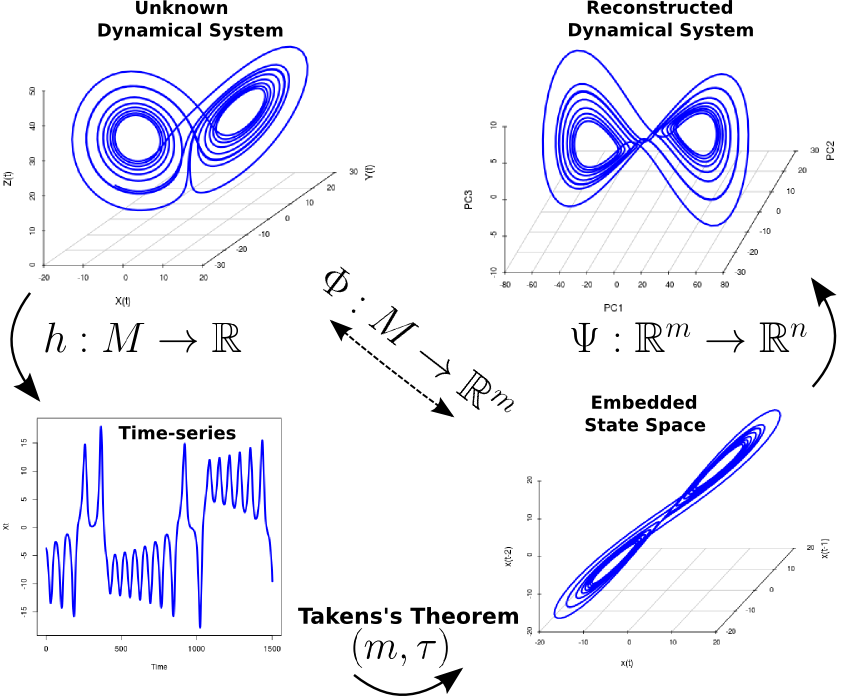
\includegraphics[width=0.95\linewidth]{images/takens_theorem_v5.png}\\}
 
  }

%%%%%%%%%%%%%%%%%%%%%%%%%%%%%%%%%%%%%%%%%%%%%%%%%%%%%%%%%%%%%%%%%%%%%%%%%%%%%%
  \headerbox{Method}{name=method,column=1,row=0}{
%%%%%%%%%%%%%%%%%%%%%%%%%%%%%%%%%%%%%%%%%%%%%%%%%%%%%%%%%%%%%%%%%%%%%%%%%%%%%%
  \indent Phase space representation of the time-delay embedded series data~\cite{mxochicale}.
  \vspace{0.5em}
     
  \noindent{\centering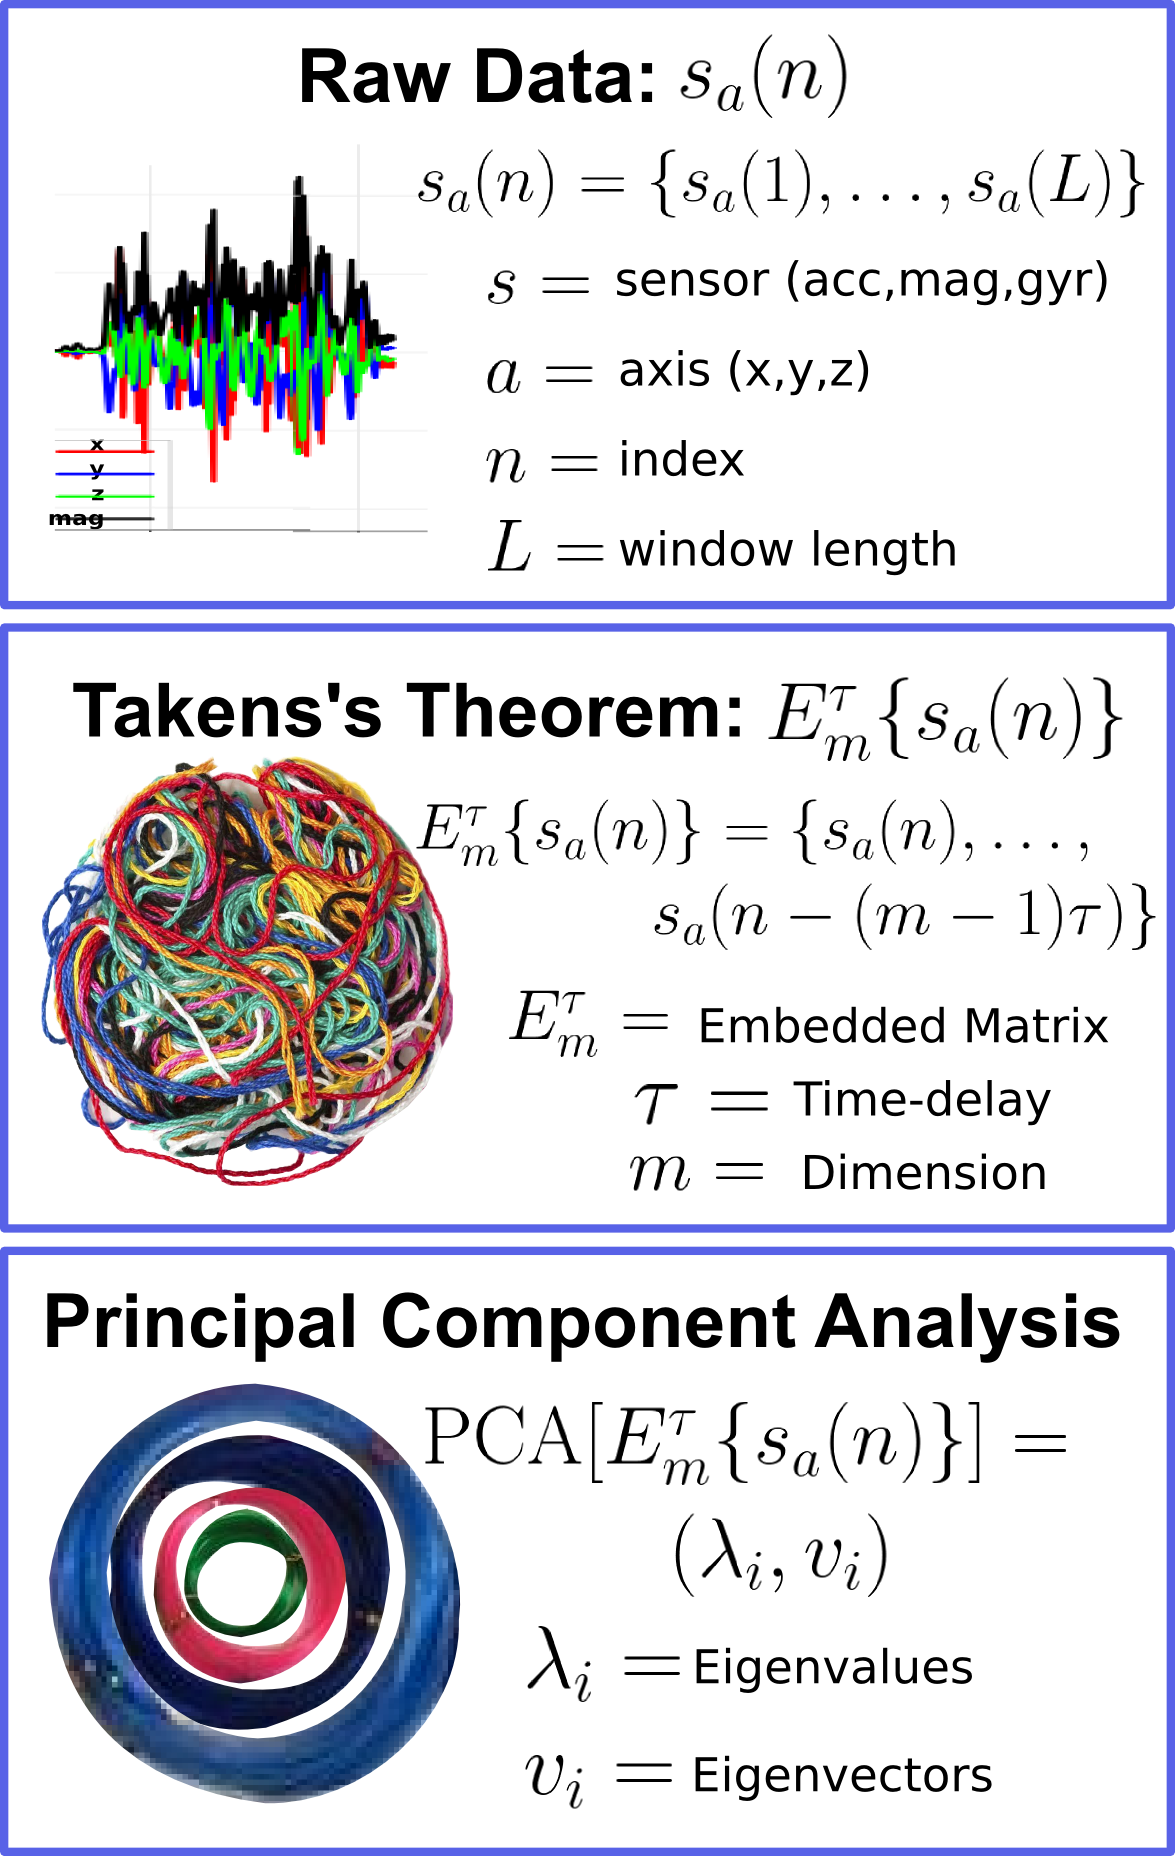
\includegraphics[width=0.95\linewidth]{images/diagram_v8.png}\\}
  
  }

%%%%%%%%%%%%%%%%%%%%%%%%%%%%%%%%%%%%%%%%%%%%%%%%%%%%%%%%%%%%%%%%%%%%%%%%%%%%%%
  \headerbox{Data Collection}{name=data,column=1,above=bottom}{
%%%%%%%%%%%%%%%%%%%%%%%%%%%%%%%%%%%%%%%%%%%%%%%%%%%%%%%%%%%%%%%%%%%%%%%%%%%%%%
Thirteen male participants with different years of experiences in dancing salsa were recruited,
one expert  (14 yr of experience), one intermediate  (4 yr of experience) and eleven novice dancers.

    \begin{multicols}{2}
	Each participant was shown a series of video clips (demonstrating salsa steps) 
	and were then asked to copy the steps in time to music during 20 seconds.
  
	\noindent{\centering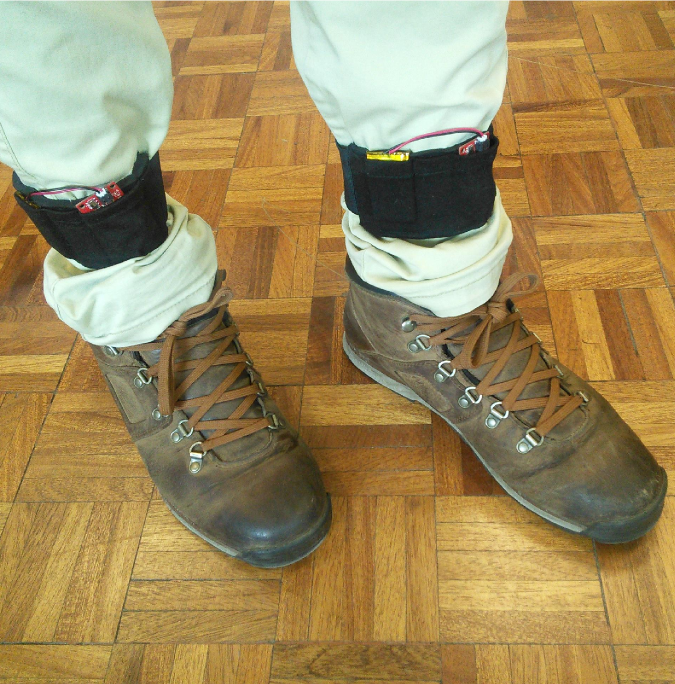
\includegraphics[width=0.95\linewidth]{images/wearingsensors_v0.png}\\}

  \end{multicols}
    
  }
  
  
  
  
%%%%%%%%%%%%%%%%%%%%%%%%%%%%%%%%%%%%%%%%%%%%%%%%%%%%%%%%%%%%%%%%%%%%%%%%%%%%%%
\headerbox{Results: Phase Space Representation}{name=results,column=2,span=2,row=0}{
  %%%%%%%%%%%%%%%%%%%%%%%%%%%%%%%%%%%%%%%%%%%%%%%%%%%%%%%%%%%%%%%%%%%%%%%%%%%%%%

  The shape of the state space show a tighter and less variated pattern for the expert than 
  for the other dexterity levels. The intermediate participant is showing a consistent action
  but this is different than the expert, and the novice is showing a pattern which appear 
  disjointed and noisy.
   \vspace{0.5em}

  \noindent{\centering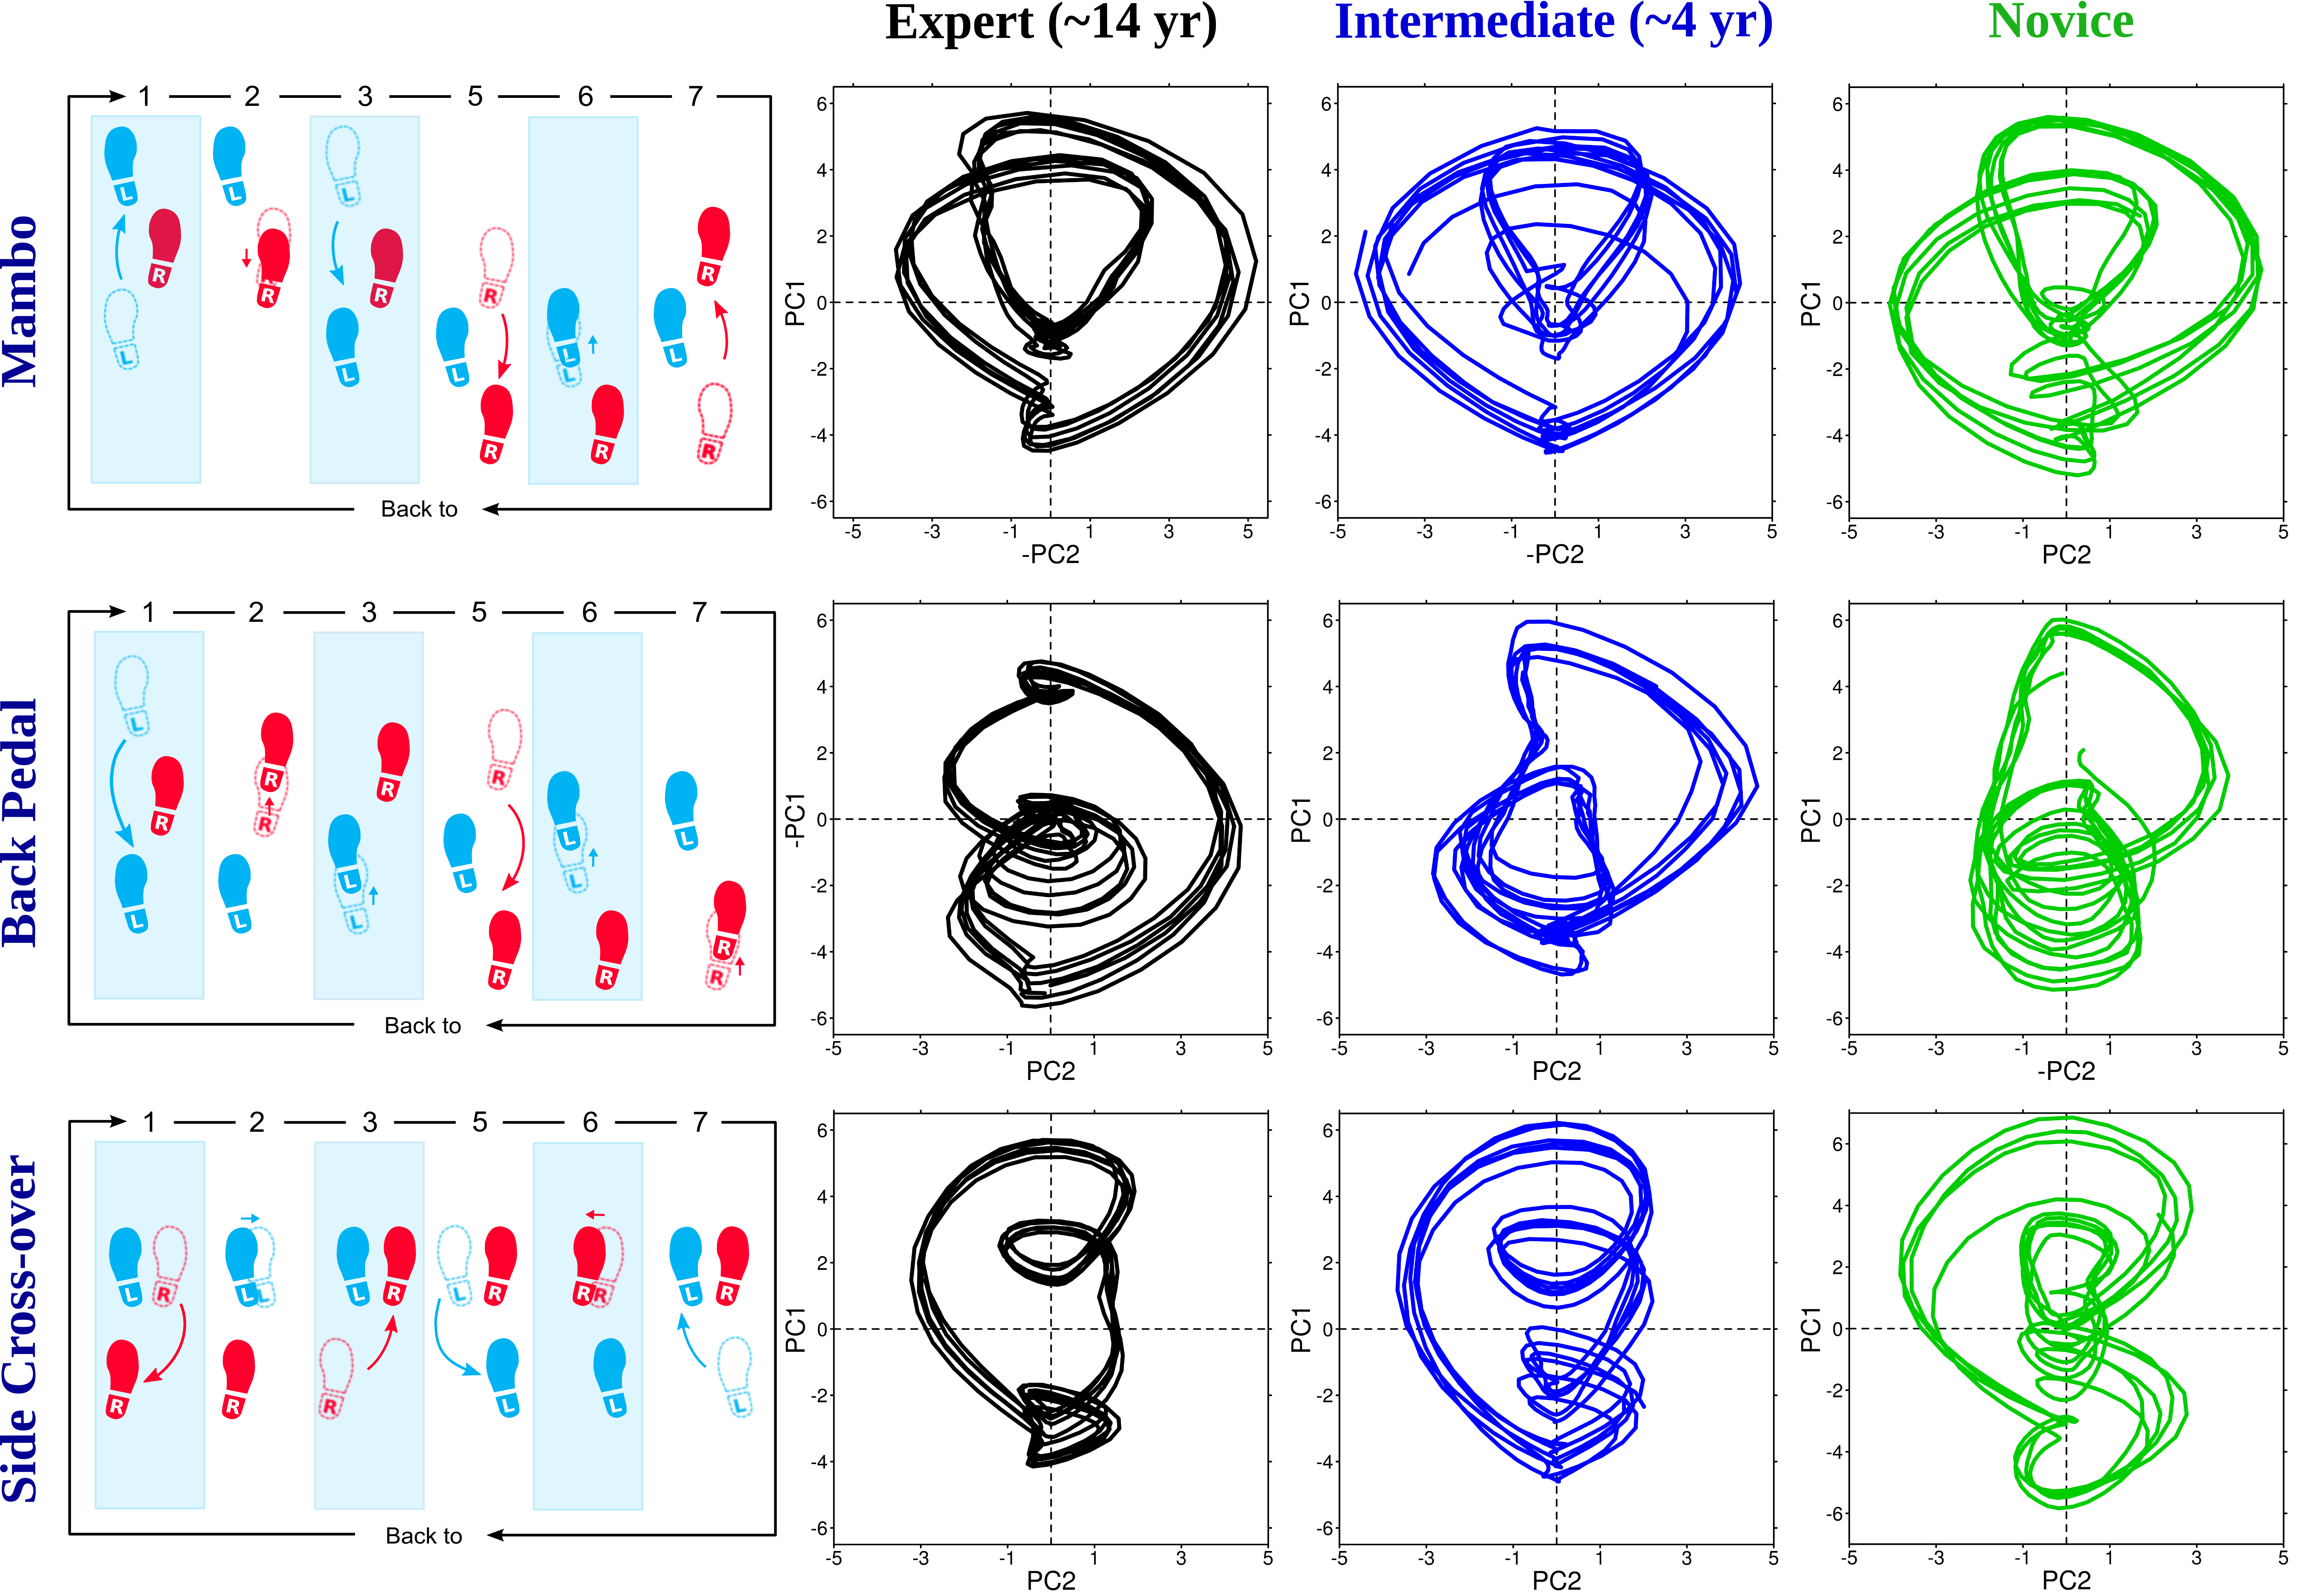
\includegraphics[width=0.95\linewidth]{images/results_v11.png}\\}

}


%%%%%%%%%%%%%%%%%%%%%%%%%%%%%%%%%%%%%%%%%%%%%%%%%%%%%%%%%%%%%%%%%%%%%%%%%%%%%%
\headerbox{Wearable Sensors}{name=ws,column=2,row=0, below=results}{
%%%%%%%%%%%%%%%%%%%%%%%%%%%%%%%%%%%%%%%%%%%%%%%%%%%%%%%%%%%%%%%%%%%%%%%%%%%%%%
\noindent{\centering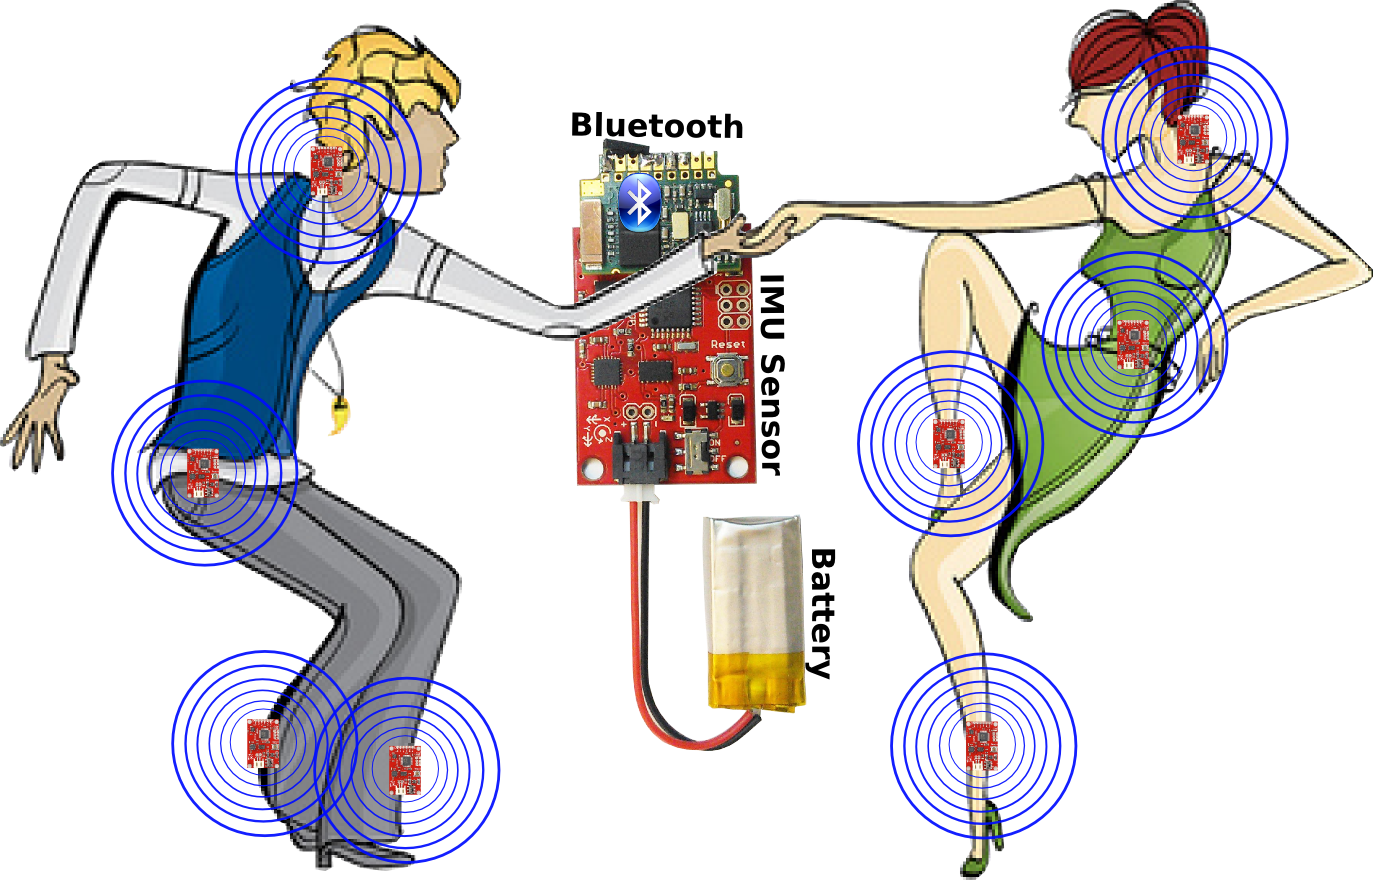
\includegraphics[width=0.95\linewidth]{images/dance_sensors_v5.png}\\}  
   \vspace{0.0em}
}

  
%%%%%%%%%%%%%%%%%%%%%%%%%%%%%%%%%%%%%%%%%%%%%%%%%%%%%%%%%%%%%%%%%%%%%%%%%%%%%%
\headerbox{Areas Of Exploitation}{name=ae,column=2,row=0, above=bottom}{
%%%%%%%%%%%%%%%%%%%%%%%%%%%%%%%%%%%%%%%%%%%%%%%%%%%%%%%%%%%%%%%%%%%%%%%%%%%%%%
\indent{}Rehabilitation, pain therapy, sports, gaming and human-robot interaction.
   \vspace{0.0em}
}

  
%%%%%%%%%%%%%%%%%%%%%%%%%%%%%%%%%%%%%%%%%%%%%%%%%%%%%%%%%%%%%%%%%%%%%%%%%%%%%%
  \headerbox{References}{name=references,column=3,above=bottom}{
%%%%%%%%%%%%%%%%%%%%%%%%%%%%%%%%%%%%%%%%%%%%%%%%%%%%%%%%%%%%%%%%%%%%%%%%%%%%%%
    \smaller
    \bibliographystyle{ieee}
    \renewcommand{\section}[2]{\vskip 0.05em}
      \begin{thebibliography}{1}\itemsep=-0.01em
      \setlength{\baselineskip}{0.4em}
      \bibitem{nhammerla11}
         N. Hammerla, T. Ploetz, P. Andras, P. Olivier
         \newblock Assessing Motor Performance with PCA
         \newblock In {\em International Workshop on Frontiers in Activity Recognition using Pervasive Sensing '11}
      \bibitem{asama13}
      	A. Sama, F. J. Ruiz, N. Agell, C. Perez-Lopez, A. Catala, J. Cabestany
       	\newblock Gait identification by means of box approximation geometry of reconstructed attractors in latent space
	\newblock In {\em Neurocomputing '13}
      \bibitem{mxochicale}
        M.~Perez-Xochicale, C.~Baber, N.~Cooke.
        \newblock 
        Dexterity Assessment for Salsa Dancers Through the Time-delay Embedded Phase Space Representation.
        \newblock Submitted to {\em ISWC '15}
      \end{thebibliography}
}

 
\headerbox{Conclusion \& Future Work}{name=conclu,column=3, below=results,above=references}{  
The phase space representation applies a model of consistency to the data for dexterity assessment.
Investigate manifold learning methods for dimensionality reduction.}
 

\end{poster}

\end{document}
